\documentclass[oneside, 11pt]{article}

\usepackage[T1]{fontenc}
\usepackage[utf8]{inputenc}
\usepackage[english]{babel}

\usepackage{fouriernc}
\usepackage[detect-all, binary-units, separate-uncertainty=true,
            per-mode=symbol, retain-explicit-plus, retain-unity-mantissa=false]{siunitx}

\usepackage{setspace}
\setstretch{1.2}

\setlength{\parskip}{\smallskipamount}
\setlength{\parindent}{0pt}

\usepackage[headheight=14pt]{geometry}
\geometry{marginparwidth=0.5cm, verbose, a4paper, tmargin=3cm, bmargin=3cm,
          lmargin=2cm, rmargin=2cm}

\usepackage{float}

\usepackage[fleqn]{amsmath}
\numberwithin{equation}{section}
\numberwithin{figure}{section}

\usepackage{graphicx}
\graphicspath{{images/}{../../../images/}}

\usepackage{tikz}
\usetikzlibrary{shapes}
\usetikzlibrary{plotmarks}

\newcounter{Exercise}
\setcounter{Exercise}{1}
\usepackage{xcolor}
\definecolor{shadecolor}{gray}{0.9}
\usepackage{framed}
\usepackage{caption}

\usepackage{url}


\usepackage{fancyhdr}
\pagestyle{fancy}
\fancyhf{}
\rhead{\thepage}
\renewcommand{\footrulewidth}{0pt}
\renewcommand{\headrulewidth}{0pt}

\fancypagestyle{firststyle}
{
    \fancyhf{}
    \rhead{\thepage}
    \cfoot{
\includegraphics[height=30pt]{HiSPARClogo}}
    \rfoot{
\includegraphics[height=25pt]{CCbysa}}
    \lfoot{
\includegraphics[height=30pt]{NIKHEFlogo}}
    \renewcommand{\footskip}{50pt}
    \renewcommand{\footrulewidth}{0.1pt}
    \renewcommand{\headrulewidth}{0pt}
}

\newcommand{\figref}[1]{Figuur~\ref{#1}}

\newcommand{\hisparc}{\textsmaller{HiSPARC}\xspace}
\newcommand{\kascade}{\textsmaller{KASCADE}\xspace}
\newcommand{\sapphire}{\textsmaller{SAPPHiRE}\xspace}
\newcommand{\jsparc}{\textsmaller{jSparc}\xspace}
\newcommand{\hdf}{\textsmaller{HDF5}\xspace}
\newcommand{\aires}{\textsmaller{AIRES}\xspace}
\newcommand{\csv}{\textsmaller{CSV}\xspace}
\newcommand{\python}{\textsmaller{PYTHON}\xspace}
\newcommand{\corsika}{\textsmaller{CORSIKA}\xspace}
\newcommand{\labview}{\textsmaller{LabVIEW}\xspace}
\newcommand{\daq}{\textsmaller{DAQ}\xspace}
\newcommand{\adc}{\textsmaller{ADC}\xspace}
\newcommand{\hi}{\textsc{h i}\xspace}
\newcommand{\hii}{\textsc{h ii}\xspace}
\newcommand{\mip}{\textsmaller{MIP}\xspace}
\newcommand{\hisparcii}{\textsmaller{HiSPARC II}\xspace}
\newcommand{\hisparciii}{\textsmaller{HiSPARC III}\xspace}

\DeclareSIUnit{\electronvolt}{\ensuremath{\mathrm{e\!\!\:V}}}

\DeclareSIUnit{\unitsigma}{\ensuremath{\sigma}}
\DeclareSIUnit{\mip}{\textsmaller{MIP}}
\DeclareSIUnit{\adc}{\textsmaller{ADC}}

\DeclareSIUnit{\gauss}{G}
\DeclareSIUnit{\parsec}{pc}
\DeclareSIUnit{\year}{yr}



\begin{document}

\title{Zonnewind}
\author{N.G. Schultheiss}
\date{}

\maketitle
\thispagestyle{firststyle}

\section{Inleiding}

Deze module volgt op de module ``De Zon'' en wordt vervolgd met
de module ``Kosmische straling''.


\section{Zonnewind}

De Zon zendt niet alleen electromagnetische straling uit, maar ook
zonnewind. De zonnewind bestaat uit deel\-tjes. Bij de kernfusie
in de Zon komen deeltjes zoals positronen en neutrino's vrij. De neutrino's
kunnen de Zon redelijk eenvoudig verlaten. Een deel van de de zonnewind
zal dus uit neutrino's bestaan. Positronen reageren vrij makkelijk
met electronen, de zonnewind zal dus vrij weinig positronen bevatten.
Als we de zonnewind onderzoeken, blijkt dat deze ook veel snel bewegende
ionen bevat. Een niet onaanzienlijk deel hiervan bestaat uit protonen
of waterstofkernen. 

In de buurt van de aarde zijn er ongeveer 10 kosmische deeltjes per
kubieke centimeter. De deeltjes vallen uiteen in twee groepen. De
deeltjes die afkomstig zijn van de polen van de zon. Deze hebben een
snelheid in de buurt van 400km/s. Verder zijn er deeltjes afkomstig
van zonnevlekken, deze hebben een snelheid in de buurt van 800km/s.


\paragraph*{Opdracht 1:}

\emph{Op een bepaald moment zien we geen zonnevlekken op de zon. Bereken
hoeveel deeltjes er in de buurt van de aarde door een oppervlak van
$1\mathrm{m}^{2}$ gaan. Een dergelijke stroom deeltjes door $1\mathrm{m}^{2}$
wordt ook wel ``flux'' genoemd.}


\section{Bewegingsenergie}

We kunnen de snelheid van de zonnewinddeeltjes meten in m/s. Meestal
wordt echter niet de snelheid, maar de energie van de zonnewinddeeltjes
gemeten. In het geval van bewegende deeltjes is dit de bewegings-
of kinetische energie. Volgens de klassieke natuurkunde kunnen we
de bewegingsenergie van een deeltje op de volgende manier afleiden:

\begin{equation}
F\triangle t=m\triangle v
\end{equation}


\begin{equation}
F=m\frac{\triangle v}{\triangle t}
\end{equation}


Nu we de kracht op een deeltje weten, kunnen we de arbeid die deze
kracht verricht berekenen:

\begin{equation}
W=Fs=m\frac{\triangle v}{\triangle t}s
\end{equation}


Omdat arbeid een vorm van energieoverdracht is, kunnen we uitrekenen
hoeveel de energie van een deeltje veranderd :

\begin{equation}
\begin{array}{c}
s=v_{gemiddeld}(t_{eind}-t_{begin})\\
\triangle E=W=m\frac{v_{eind}-v_{begin}}{t_{eind}-t_{begin}}v_{gemiddeld}(t_{eind}-t_{begin})
\end{array}
\end{equation}


\begin{equation}
E_{eind}-E_{begin}=m(v_{eind}-v_{begin})\frac{v_{begin}+v_{eind}}{2}
\end{equation}


We nemen $E_{begin}=0\mathrm{J}$, $v_{begin}=0\frac{\mathrm{m}}{s}$.

\begin{equation}
E_{eind}=mv_{eind}\frac{v_{eind}}{2}
\end{equation}


Generalizeren geeft:

\begin{equation}
E=\frac{1}{2}mv^{2}
\end{equation}


\paragraph*{Opdracht 2:}

\emph{Bereken de energie van een proton of waterstofkern met een massa
van} $1.67262158*10^{-27}$kg \emph{en een snelheid van} 400km/s.

Omdat de energie in J of Joule wordt uitgedrukt, krijgen we een heel
klein getal. Meestal wordt de energie van deze deeltjes uitgedrukt
in eV of electronVolt. Een volt is een maat voor de electrische energie
per lading:

\begin{equation}
1\mathrm{V}=\frac{1\mathrm{J}}{1\mathrm{C}}
\end{equation}


\begin{equation}
1\mathrm{V}*1\mathrm{C}=1\mathrm{J}
\end{equation}


De elementaire lading $e=1.60217646*10^{-19}$C. 

\begin{equation}
1e\mathrm{V}=1.60217646*10^{-19}\mathrm{C*1V}=1.60217646*10^{-19}\mathrm{J}
\end{equation}


\paragraph*{Opdracht 3:}

\emph{Bereken de energie van een proton of waterstofkern met een massa
van} $1.67262158*10^{-27}$kg \emph{en een snelheid van} 400km/s \emph{in}
eV.


\section{Magnetische velden.}


\subsection{Ladingen in magnetische velden}

\begin{figure}[h]
\noindent \begin{centering}
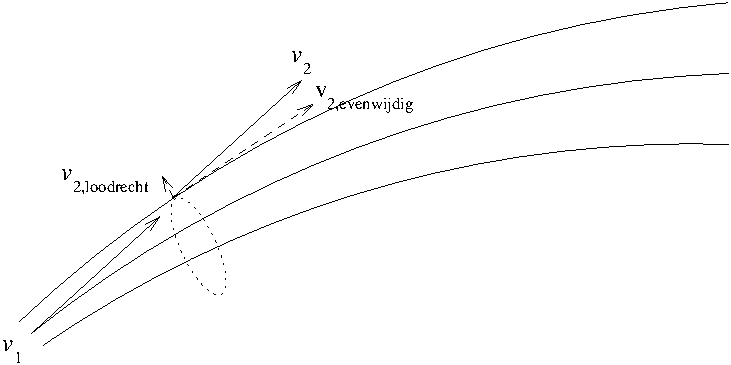
\includegraphics[scale=0.75]{lorentz}
\par\end{centering}

\caption{De Lorentzkracht in een divergerend veld}
\end{figure}


Als een lading in een magnetisch veld beweegt, ondervindt deze een
Lorentzkracht loodrecht op de bewegingsrichting en de magnetische
veldlijnen. Als een geladen deeltje met een snelheid $v_{1}$ langs
een kromme veldlijn beweegt, zal dit deeltje in eerste instantie rechtdoor
gaan. Helaas wijkt de richting van de snelheid steeds meer af van
de richting van de veldlijn. We kunnen de snelheid dan ontbinden in
een component $v_{2,\mathrm{evenwijdig}}$ langs de veldlijn en een
component $v_{2,\mathrm{loodrecht}}$ loodrecht op de veldlijn. De
component loodrecht op de veldlijn en het magnetisch veld veroorzaken
dan een Lorentzkracht. Het deeltje wil dan een beetje in de richting
van de gestippelde cirkel bewegen. Omdat er ook nog een snelheid in
de richting van de veldlijn is, begint het deeltje rond de veldlijn
te spiraliseren.


\subsection{De Zon}

\begin{figure}[h]
\noindent \begin{centering}
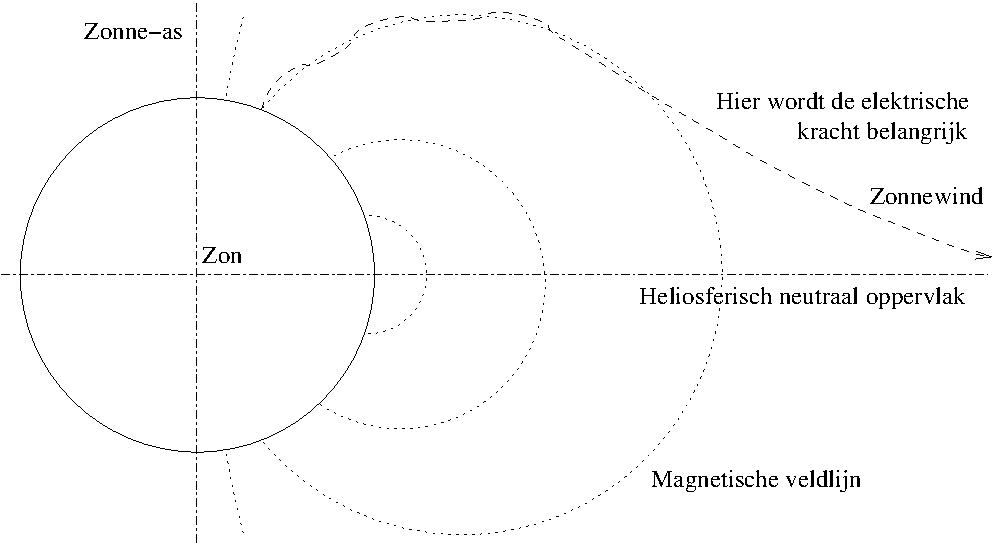
\includegraphics[scale=0.75]{baan}
\par\end{centering}

\caption{Zonnewind zonder zonnevlekken in de omgeving van de zon}
\end{figure}


De zon heeft evenals de aarde een magnetisch veld. Het magnetisch
veld van de aarde keert af en toe om, in de afgelopen 2.000.000 jaar
is dit 7 keer gebeurt. Bij de zon gebeurt dit om de 7 tot 15 jaar. 

Als er geen zonnevlekken zijn hoeven we alleen met het magnetisch
veld langs de zonne-as rekening te houden. Als een geladen deeltje
door een magnetisch veld beweegt, ontstaat er een kracht die zorgt
dat het deeltje wordt afgebogen. Deze kracht staat loodrecht op het
veld en loodrecht op de snelheid van het deeltje. De geladen deeltjes
hebben daarom de neiging om globaal langs de magnetische veldlijnen
te spiraliseren.

Naast de magnetische kracht werkt er ook een elektrische kracht op
de deeltjes. Deeltjes met een gelijke lading stoten elkaar af. Omdat
de deeltjes zowel van de Noord- als van de Zuidpool afkomstig zijn,
is deze elektrische kracht op eenafstand van 3 maal de straal van
de Zon niet meer te verwaarlozen. De deeltjes bewegen nu globaal in
het vlak door de equator van de Zon, het heliosferisch neutraal oppervlak.

In het geval van zonnevlekken zijn er extra magnetische velden op
de zon. Bij ieder zonnevlek is een magnetische pool te vinden. Het
komt voor dat langs de veldlijnen van pool naar pool een gloeiend
hete massa stroomt, een zonnevlam. Deze massa is echter kouder dan
het gas van de fotosfeer. Als je boven op een zonnevlam kijkt, zie
je een donkere vlek, een zonnevlek. Als er zonnevlekken zijn worden
er ook zonnestralingsdeeltjes waargenomen met een snelheid van 800km/s.


\paragraph*{Opdracht 4:}

\emph{Bereken de energie in }eV\emph{ als we aannemen dat deze deeltjes
snelle protonen zijn. }


\subsection{De Aarde}

Omdat de Aarde ook in dit vlak beweegt, komen deze deeljes voor een
deel op de Aarde. De lichte elektronen worden het eerst ingevangen
in het magnetisch veld van de Aarde. Deze vormen de buitenste van
Allen gordel. Zwaardere deeltjes, zoals protonen, hebben een grotere
kracht nodig om af te buigen. Deze vliegen verder in het veld van
de Aarde en vormen de binnenste van Allen gordel.

Een klein deel van de deeltjes wordt afgebogen en komt via de polen
naar het Aardoppervlak. Omdat dit een convergerend veld is worden
de deeltjes afgeremd. Rond de magnetische Zuid- en Noordpool van de
Aarde komen deze deeltjes tot in de atmosfeer. De energie wordt hier
door botsingen met de atomen in de atmosfeer omgezet in de Aurora
Borealis of het poollicht. 

Als er heel snelle geladen deeltjes in de richting van de Aarde bewegen,
zal de straal van de baan zo groot worden dat de deeltjes het aardoppervlak
bereiken. Deze deeltjes kunnen met een detector worden waargenomen.

\end{document}
